El nivel supervisor constituye la capa de coordinación del sistema, responsable de orquestar tareas complejas que requieren la integración de múltiples subsistemas. A diferencia del nivel regulatorio que ejecuta comandos individuales, el supervisor planifica secuencias completas de acciones para lograr objetivos de alto nivel.\\

Responsabilidades principales:

\begin{itemize}[label=$\bullet$]
    \item Planificación de secuencias: descompone tareas complejas en secuencias ordenadas de comandos básicos
    \item Gestión de estado global: mantiene información sobre posición acumulada, dimensiones del workspace, mapas de ubicaciones
    \item Integración con visión: invoca algoritmos de procesamiento de imágenes e interpreta sus resultados
    \item Comunicación bidireccional: envía comandos al nivel regulatorio y procesa respuestas asíncronas
    \item Persistencia de información: guarda datos críticos en archivos JSON que sobreviven reinicios
\end{itemize}

Modelo de ejecución orientado a eventos:\\
\noindent
El supervisor utiliza un modelo orientado a eventos mediante callbacks. Cuando envía un comando de movimiento, registra un callback que será invocado cuando llegue el mensaje de completado. Durante la espera, el bucle principal continúa procesando otros eventos. Este diseño evita bloqueos y permite respuesta inmediata a eventos inesperados.

\subsubsection{Procesos implementados}

El sistema implementa cuatro procesos principales que coordinan movimientos, captura de imágenes y ejecución de algoritmos de visión.

\underline{Proceso 1: homing (referenciado del sistema):} Establece el origen del sistema de coordenadas moviendo los ejes hasta los finales de carrera y retrocediendo offsets calibrados.

\begin{table}[H]
\centering
\small
\begin{tabular}{|l|p{10cm}|}
\hline
Paso & Acción \\
\hline
1. Verificación inicial & Confirma que el brazo está en posición de movimiento. Si no lo está, ejecuta transición antes de continuar. \\
\hline
2. Configuración & Reduce velocidades a velocidades de homing (más lentas para evitar impactos bruscos). \\
\hline
3. Homing horizontal & Mueve hacia la derecha hasta activar final de carrera. Retrocede offset calibrado. \\
\hline
4. Homing vertical & Mueve hacia arriba hasta activar final de carrera. Retrocede offset calibrado. \\
\hline
5. Establecer origen & Establece la posición actual como (0,0) en firmware y supervisor. \\
\hline
6. Restauración & Restaura velocidades normales. \\
\hline
7. Persistencia & Guarda la referencia en archivo JSON con timestamp. \\
\hline
\end{tabular}
\caption{\textit{Secuencia del proceso de homing}}
\label{tab:proceso_homing}
\end{table}

\underline{Proceso 2: calibración del espacio de trabajo:} Mide las dimensiones útiles del espacio de trabajo moviendo los ejes hasta sus límites opuestos.

\begin{table}[H]
\centering
\small
\begin{tabular}{|l|p{10cm}|}
\hline
Paso & Acción \\
\hline
1. Homing inicial & Ejecuta proceso de homing para partir desde origen conocido. \\
\hline
2. Medición horizontal & Mueve hacia la izquierda hasta activar límite. Registra distancia recorrida. \\
\hline
3. Retorno horizontal & Vuelve cerca del origen horizontal. \\
\hline
4. Medición vertical & Mueve hacia abajo hasta activar límite. Registra distancia recorrida. \\
\hline
5. Cálculo de dimensiones & Resta márgenes de seguridad (5-10mm) para obtener dimensiones útiles. \\
\hline
6. Homing final & Ejecuta homing nuevamente para volver al origen. \\
\hline
7. Persistencia & Guarda dimensiones en archivo JSON. \\
\hline
\end{tabular}
\caption{\textit{Secuencia del proceso de calibración}}
\label{tab:proceso_calibracion}
\end{table}

\underline{Proceso 3: mapeo del entorno:} Escanea el workspace para detectar posiciones de tubos (coordenadas Y) y plantas (coordenadas X), generando mapas que guían la navegación posterior.

\begin{table}[H]
\centering
\small
\begin{tabular}{|l|p{10cm}|}
\hline
Paso & Acción \\
\hline
1. Escaneo vertical & Mueve el eje vertical en pasos incrementales. En cada pausa, captura imagen y ejecuta detector de tubos. Registra coordenadas Y donde detecta tubos. \\
\hline
2. Guardado de tubos & Ordena y guarda las coordenadas Y detectadas en archivo JSON. \\
\hline
3. Escaneos horizontales & Para cada tubo: se posiciona en su coordenada Y, ejecuta barrido horizontal detectando cintas negras, registra coordenadas X de detecciones. \\
\hline
4. Guardado de cintas & Guarda las coordenadas X por tubo en archivo JSON. \\
\hline
5. Retorno & Mueve el sistema de vuelta al origen (0,0). \\
\hline
\end{tabular}
\caption{\textit{Secuencia del proceso de mapeo}}
\label{tab:proceso_mapeo}
\end{table}

\underline{Proceso 4: cosecha interactiva:} Navega a cada posición registrada, clasifica la planta, y si está madura ejecuta la recolección.

\begin{table}[H]
\centering
\small
\begin{tabular}{|l|p{10cm}|}
\hline
Paso & Acción \\
\hline
1. Carga de mapas & Lee archivos JSON con posiciones de tubos y cintas. Genera lista de posiciones (X,Y) a visitar. \\
\hline
2. Navegación & Para cada posición: mueve el sistema XY a esa coordenada, espera confirmación de llegada. \\
\hline
3. Clasificación & Captura imagen. Ejecuta clasificador morfológico que retorna clase predicha y confianza. \\
\hline
4. Decisión & Si clase es lechuga: ejecuta corrección de posición, extiende brazo, cierra gripper, eleva planta. \\
\hline
5. Depósito & Si tiene planta en gripper: navega a zona de depósito, inclina brazo, abre gripper. \\
\hline
6. Continuación & Procesa siguiente posición o finaliza si no quedan. \\
\hline
7. Finalización & Vuelve al origen. Registra estadísticas: plantas cosechadas, vasos vacíos, plantas inmaduras. \\
\hline
\end{tabular}
\caption{\textit{Secuencia del proceso de cosecha interactiva}}
\label{tab:proceso_cosecha}
\end{table}

Manejo de errores durante procesos:\\
Durante la ejecución de cualquier proceso, el supervisor monitorea eventos inesperados:

\begin{itemize}[label=$\bullet$]
    \item \underline{Límite activado inesperadamente}: detiene el proceso, registra el error, y preserva el estado para diagnóstico
    \item \underline{Pérdida de comunicación}: si un comando no recibe respuesta en tiempo límite, aborta el proceso e intenta re-establecer comunicación
    \item \underline{Fallo de detector}: si un algoritmo de visión no retorna resultados válidos, registra la falla e intenta continuar o solicita intervención
\end{itemize}

\begin{figure}[H]
    \centering
    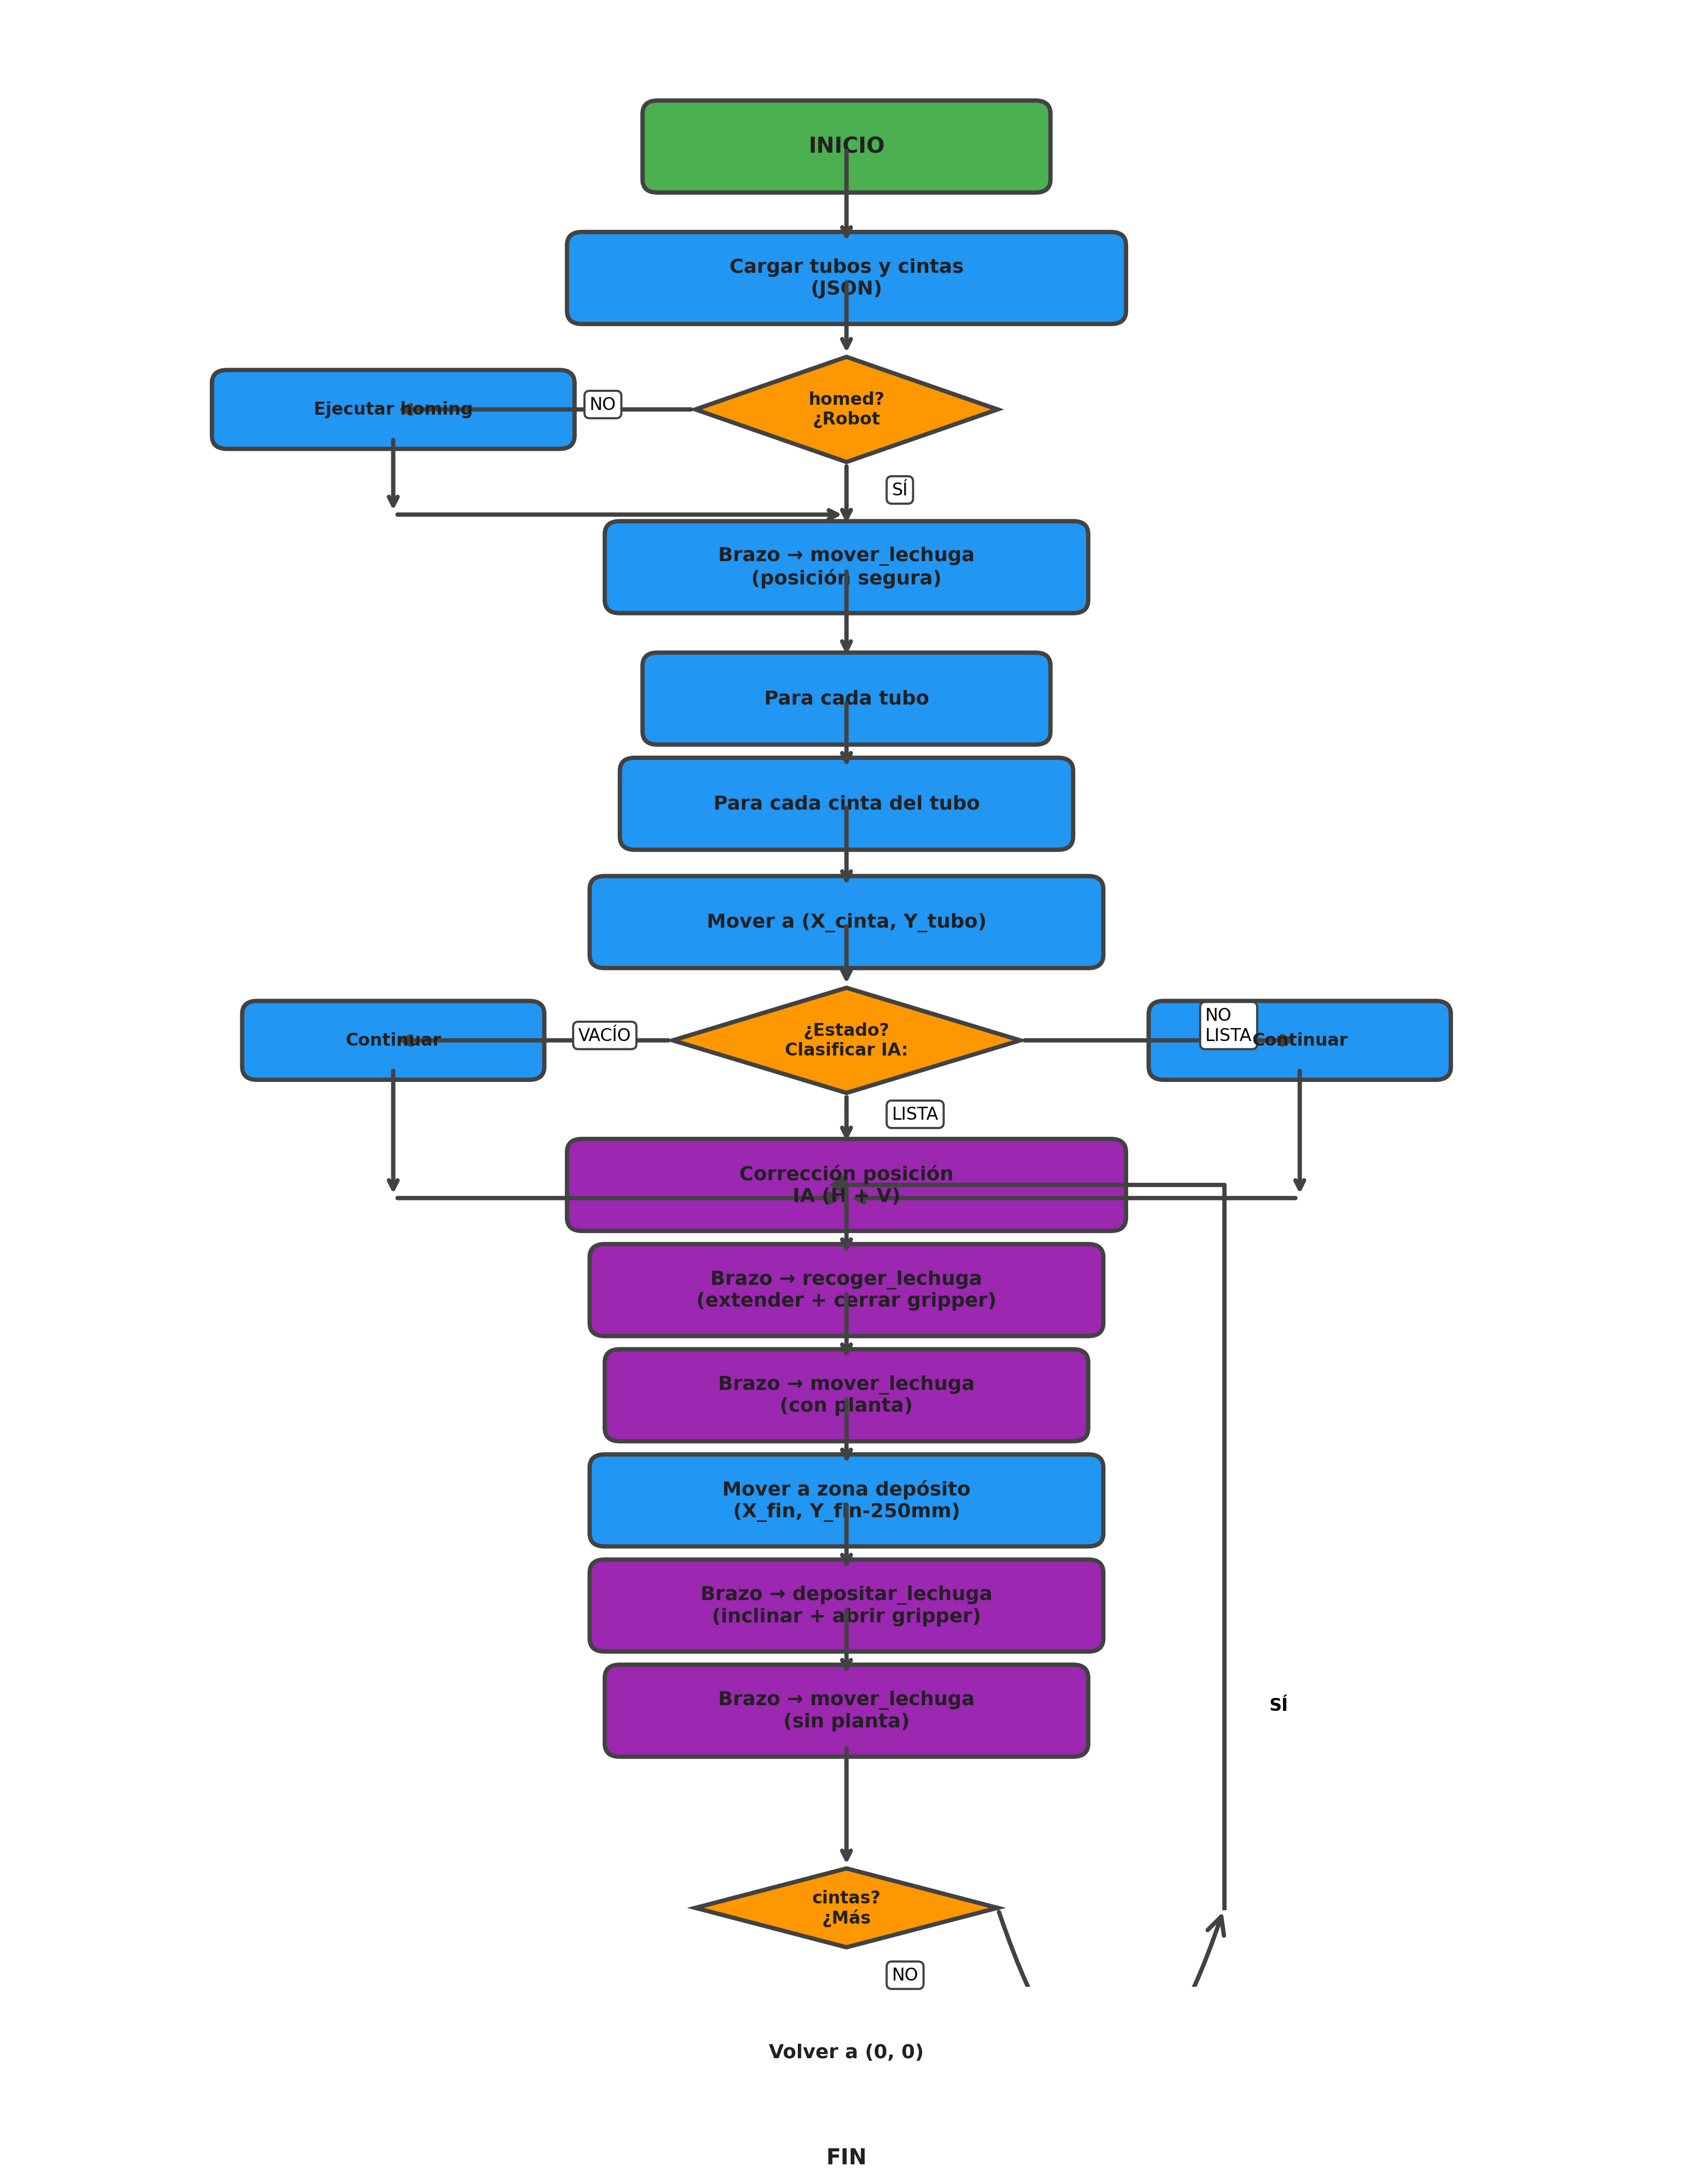
\includegraphics[width=0.3\textwidth]{imagenes/diagrama_flujo_cosecha.png}
    \caption{\textit{Diagrama de flujo detallado del proceso de cosecha mostrando decisiones según clasificación}}
    \label{fig:flujo_cosecha}
\end{figure}
